%%%%%%%%%%%%%%%%%%%%%%%%%%%%%%%%%%%%%%%%%%%%%%%%%%%%%%%%%%%%%%%%%%%%%%%%%%%%%%%
%% SOCIOL 723 -- Social Statistics II
%% Week 1: The Linear Model and OLS  --  SANS-SERIF VARIANT (text + math)
%% Wenhao Jiang, Duke University, Fall 2026
%%%%%%%%%%%%%%%%%%%%%%%%%%%%%%%%%%%%%%%%%%%%%%%%%%%%%%%%%%%%%%%%%%%%%%%%%%%%%%%

\documentclass[aspectratio=169,11pt,xcolor=dvipsnames]{beamer}
\mode<presentation>

%% ---- fonts: Latin Modern SANS, for BOTH text and math ----------------------
%% This is the sans experiment: identical to slides.tex in every other respect.
\usepackage[T1]{fontenc}
\usepackage{lmodern}
\renewcommand{\familydefault}{\sfdefault}
\usepackage{sansmath}
\AtBeginDocument{\sansmath}

%% ---- packages --------------------------------------------------------------
\usepackage{amsmath,amsfonts,amssymb,bm}
\usepackage{graphicx}
\usepackage{booktabs}
\usepackage{tikz}
\usetikzlibrary{arrows.meta,positioning,calc}
\usepackage[english]{babel}

%% lightweight citation macros (beamer + natbib do not play well together)
\newcommand{\srcp}[1]{{\scriptsize\color{gray}(#1)}}   %% parenthetical
\newcommand{\srct}[1]{#1}                               %% inline / narrative

\DeclareMathOperator*{\argminop}{arg\,min}
\DeclareMathOperator*{\argmaxop}{arg\,max}
%% \limits forces the subscript underneath even in inline math
\newcommand{\argmin}{\argminop\limits}
\newcommand{\argmax}{\argmaxop\limits}
\DeclareMathOperator{\Cov}{Cov}
\DeclareMathOperator{\Var}{Var}
\DeclareMathOperator{\Corr}{Corr}
\DeclareMathOperator{\trace}{tr}
\DeclareMathOperator{\rank}{rank}
\DeclareMathOperator{\pcol}{col}
\newcommand{\indep}{\perp\!\!\!\perp}

%% ---- notation conventions (course-wide) ------------------------------------
%%  \E   population expectation (plain italic E)
%%  \En  sample / empirical expectation (blackboard-bold E)
%%  matrices and vectors are BOLD ITALIC via \bm, so they sit naturally
%%  alongside the italic scalar notation
\newcommand{\E}{E}
\newcommand{\En}{\mathbb{E}_n}
\newcommand{\R}{\mathbb{R}}
\newcommand{\X}{\bm{X}}
\newcommand{\Y}{\bm{y}}
\newcommand{\Ix}{\bm{I}}
\newcommand{\zero}{\bm{0}}
\newcommand{\one}{\bm{1}}
\newcommand{\Pm}{\bm{P}}
\newcommand{\Mm}{\bm{M}}
\newcommand{\bhat}{\hat{\bm{\beta}}}
\newcommand{\ehat}{\hat{\bm{e}}}

%% ---- theme -----------------------------------------------------------------
\usetheme{default}
%% thin single-line header: clickable section names, current one highlighted.
%% (miniframes is deliberately not used: one dot per slide wraps to 4 rows here)
\setbeamerfont{section in head/foot}{size=\tiny}
\setbeamertemplate{headline}{%
  \begin{beamercolorbox}[wd=\paperwidth,ht=2.4ex,dp=1.1ex,%
                         leftskip=.3cm,rightskip=.3cm]{section in head/foot}%
    \usebeamerfont{section in head/foot}%
    \insertsectionnavigationhorizontal{.94\paperwidth}{}{}%
  \end{beamercolorbox}%
}

\definecolor{dukeblue}{RGB}{1,33,105}
\definecolor{accent}{RGB}{200,78,0}
\definecolor{softgray}{RGB}{242,242,245}

\setbeamercolor{structure}{fg=dukeblue}
\setbeamercolor{frametitle}{fg=dukeblue,bg=white}
\setbeamercolor{section in head/foot}{fg=white,bg=dukeblue}
\setbeamercolor{section in head/foot shaded}{fg=white!50!dukeblue,bg=dukeblue}
\setbeamercolor{alerted text}{fg=accent}
\setbeamercolor{block title}{fg=white,bg=dukeblue}
\setbeamercolor{block body}{fg=black,bg=softgray}
\setbeamercolor{block title alerted}{fg=white,bg=accent}
\setbeamercolor{block body alerted}{fg=black,bg=softgray}

\setbeamertemplate{footline}[page number]
\setbeamertemplate{navigation symbols}{}
%% continued frames keep the SAME font size and spill onto a new slide
\setbeamertemplate{frametitle continuation}{\normalfont\footnotesize\ (cont.)}
\setbeamertemplate{itemize items}[circle]
\setbeamertemplate{blocks}[rounded][shadow=false]
\setbeamerfont{frametitle}{series=\bfseries}
\setbeamerfont{footnote}{size=\scriptsize}
\setbeamerfont{caption}{size=\footnotesize}
\setbeamertemplate{subsection in head/foot}{}
\setbeamertemplate{subsection in head/foot shaded}{}
\setbeamertemplate{caption}[numbered]

%% marker for material that is for understanding, not for examination
\newcommand{\adv}{\,\raisebox{0.6pt}{\textcolor{accent}{$\bigstar$}}}

%% section / subsection dividers
\setbeamertemplate{section page}{%
  \begin{centering}\vfill
  {\usebeamercolor[fg]{structure}\Large\bfseries\insertsectionhead\par}
  \vskip4pt{\color{dukeblue}\rule{0.35\linewidth}{1pt}\par}
  \vfill\end{centering}}
\setbeamertemplate{subsection page}{%
  \begin{centering}\vfill
  {\usebeamercolor[fg]{structure}\large\bfseries\insertsubsectionhead\par}
  \vfill\end{centering}}


%% tighter vertical rhythm: math-heavy beamer frames otherwise overflow
\AtBeginDocument{%
  \setlength{\abovedisplayskip}{5pt}%
  \setlength{\belowdisplayskip}{5pt}%
  \setlength{\abovedisplayshortskip}{2pt}%
  \setlength{\belowdisplayshortskip}{3pt}%
}
\setbeamertemplate{frametitle}{%
  \vskip4pt\usebeamerfont{frametitle}\usebeamercolor[fg]{frametitle}%
  \insertframetitle\par\vskip2pt}
\setbeamersize{text margin left=0.75cm, text margin right=0.75cm}

%% ---- title -----------------------------------------------------------------
\title[SOCIOL 723]{SOCIOL 723: Social Statistics II\\[2pt]}
\subtitle{\large Week 1, The Linear Model and OLS\\[-8pt]}
\author[Jiang]{\large Wenhao Jiang\vspace{-1.5em}}
\institute[Duke]{}
\titlegraphic{
\includegraphics[height=1.3cm]{../Misc/duke_logo.png}}
\date{\large Department of Sociology, Fall 2026}

\begin{document}

\begin{frame}[plain]
  \titlepage
\end{frame}

\begin{frame}{Today}
  \tableofcontents
\end{frame}

%%%%%%%%%%%%%%%%%%%%%%%%%%%%%%%%%%%%%%%%%%%%%%%%%%%%%%%%%%%%%%%%%%%%%%%%%%%%%%%
\section[Orientation]{Orientation}
%%%%%%%%%%%%%%%%%%%%%%%%%%%%%%%%%%%%%%%%%%%%%%%%%%%%%%%%%%%%%%%%%%%%%%%%%%%%%%%
\begin{frame}\sectionpage\end{frame}

\begin{frame}{Three Pillars of this Course}
\begin{itemize}\itemsep6pt
  \item \textbf{Estimation} (Weeks 1--4). What is the estimator, and what are its
        statistical properties? OLS, then maximum likelihood as the general engine.
  \item \textbf{Causal inference} (Weeks 5--11). What quantity are we after, and
        what would have to be true for our estimate to recover it?
  \item \textbf{Machine learning} (Weeks 12--13). What do we do when the number of
        covariates is large and the functional form is unknown?
\end{itemize}
\vskip8pt
\begin{block}{The through-line}
Nearly everything in this course is some version of one idea:
\emph{compare units that are alike in all the ways that matter}. Regression is the
first and most transparent implementation of that idea.
\end{block}
\end{frame}

\begin{frame}{How to Read These Slides}
\begin{alertblock}{The \adv{} convention}
A frame title marked with \adv{} contains material that is here \emph{for your
understanding}, not for evaluation. Derivations in matrix form, projection
geometry, and asymptotic arguments all fall in this category.
\end{alertblock}
\vskip4pt
\begin{itemize}\itemsep4pt
  \item \textbf{What I will examine}: the \alert{scalar} versions of everything, 
        the algebra you can do by hand with $\sum_i$ signs, plus interpretation,
        assumptions, and knowing which tool fits which problem.
  \item \textbf{What is here anyway}: the general, abstract versions. You should
        read them, and you will meet them again in the literature. You will not be
        asked to reproduce them under time pressure.
  \item My slides are deliberately dense so that they work as a reference after
        class. Stop me whenever something is unclear; that is what lecture is for.
\end{itemize}
\end{frame}

\begin{frame}{What You Already Know: Model Comparison}
In \textit{Social Statistics I} you compared a \textbf{compact} model to an
\textbf{augmented} model:
\begin{align*}
  \text{MODEL C:}\quad Y_i &= \beta_0 + \beta_1 X_{1i} + \epsilon_i \\
  \text{MODEL A:}\quad Y_i &= \beta_0 + \beta_1 X_{1i} + \beta_2 X_{2i} + \epsilon_i
\end{align*}
and asked whether the extra parameters bought enough reduction in error:
\begin{align*}
  PRE = \frac{SSE_C - SSE_A}{SSE_C},
  \qquad
  F = \frac{(SSE_C - SSE_A)/(PA - PC)}{SSE_A/(n - PA)}.
\end{align*}
\pause
\begin{itemize}
  \item All of this stays. Today we look \emph{inside} the estimator: where do
        $\hat\beta_0,\hat\beta_1$ come from, and what do they mean?
  \item Then we rewrite it in matrix form, which is the language the rest of the
        course speaks.
\end{itemize}
\end{frame}

\begin{frame}{Notation We Will Use All Semester}
\begin{block}{Population versus sample}
\begin{align*}
  \E[\,\cdot\,] &: \text{the \textbf{population} expectation, a fixed, unknown number} \\[3pt]
  \En[\,\cdot\,] &\equiv \frac{1}{n}\sum_{i=1}^{n} (\,\cdot\,)
  : \text{the \textbf{sample} (empirical) expectation, a random variable}
\end{align*}
\end{block}
\vskip2pt
\begin{itemize}\itemsep3pt
  \item Greek letters ($\beta$, $\sigma$, $\epsilon$) are \emph{population}
        quantities we never observe; hats ($\hat\beta$, $\hat e$) are \emph{sample}
        quantities we compute.
  \item $\epsilon_i$ always denotes the error term; $\hat e_i$ the fitted residual.
        They are different objects, and confusing them is the single most common
        source of trouble.
  \item Later: $\bm{\text{bold italic}}$ $=$ vector or matrix (lowercase
        $\Y$ for vectors, uppercase $\X$ for matrices), $'$ $=$ transpose.
\end{itemize}
\vskip2pt
The whole of statistical inference is the study of the gap between $\E$ and $\En$.
\end{frame}

%%%%%%%%%%%%%%%%%%%%%%%%%%%%%%%%%%%%%%%%%%%%%%%%%%%%%%%%%%%%%%%%%%%%%%%%%%%%%%%
\section[Scalar OLS]{OLS in Scalar Form}
%%%%%%%%%%%%%%%%%%%%%%%%%%%%%%%%%%%%%%%%%%%%%%%%%%%%%%%%%%%%%%%%%%%%%%%%%%%%%%%
\begin{frame}\sectionpage\end{frame}

\subsection*{The Bivariate Model}
\begin{frame}\subsectionpage\end{frame}

\begin{frame}{The Bivariate Linear Model}
For each unit $i = 1,\dots,n$ we observe an outcome $Y_i$ and one regressor $X_i$:
\begin{align*}
  Y_i = \beta_0 + \beta_1 X_i + \epsilon_i .
\end{align*}
\begin{itemize}\itemsep4pt
  \item $\beta_0$, the \textbf{intercept}: the average of $Y$ when $X = 0$.
  \item $\beta_1$, the \textbf{slope}: how much higher $Y$ is, on average, for
        units that differ by one unit in $X$.
  \item $\epsilon_i$, the \textbf{error}: everything else that makes unit $i$'s
        outcome differ from the line.
\end{itemize}
\vskip6pt
\begin{block}{Running example, all semester}
GSS 2010--2022, full-time workers aged 25--64 ($n = 3{,}509$). \\
$Y_i = $ log personal earnings, $X_i = $ years of schooling completed.
\end{block}
\end{frame}

\begin{frame}{The Least Squares Criterion}
We do not observe $\beta_0,\beta_1$. We pick estimates $b_0, b_1$ to make the
fitted line as close as possible to the data. ``Close'' $=$ small squared
vertical distances:
\begin{align*}
  S(b_0, b_1) \;=\; \sum_{i=1}^{n}\big(Y_i - b_0 - b_1 X_i\big)^2 .
\end{align*}
\pause
\begin{itemize}\itemsep4pt
  \item Why squares? They punish large misses more than small ones, they make the
        problem differentiable, and, as we will see, they deliver the
        conditional \emph{mean}.
  \item Why vertical? Because we are predicting $Y$ from $X$, not the reverse.
        Regressing $X$ on $Y$ gives a different line.
\end{itemize}
\vskip4pt
The OLS estimates are $(\hat\beta_0, \hat\beta_1) = \argmin_{b_0,b_1} S(b_0,b_1)$.
\end{frame}

\begin{frame}{Step 1: The First-Order Conditions}
$S$ is a smooth, convex function of two numbers. Set both partial derivatives to
zero. Using the chain rule,
\begin{align*}
  \frac{\partial S}{\partial b_0}
  &= \sum_{i=1}^n 2\big(Y_i - b_0 - b_1X_i\big)\cdot(-1)
  \ \overset{!}{=}\ 0 ,\\[4pt]
  \frac{\partial S}{\partial b_1}
  &= \sum_{i=1}^n 2\big(Y_i - b_0 - b_1X_i\big)\cdot(-X_i)
  \ \overset{!}{=}\ 0 .
\end{align*}
Dividing by $-2$ gives the two \alert{normal equations}:
\begin{align*}
  \sum_i \big(Y_i - \hat\beta_0 - \hat\beta_1 X_i\big) &= 0 , \tag{N1}\\
  \sum_i X_i\big(Y_i - \hat\beta_0 - \hat\beta_1 X_i\big) &= 0 . \tag{N2}
\end{align*}
\end{frame}

\begin{frame}{What the Normal Equations Say}
Write $\hat e_i = Y_i - \hat\beta_0 - \hat\beta_1 X_i$ for the fitted residual. Then
\begin{align*}
  \text{(N1)}: \quad \sum_i \hat e_i = 0
  \qquad\qquad
  \text{(N2)}: \quad \sum_i X_i \hat e_i = 0 .
\end{align*}
\begin{itemize}\itemsep5pt
  \item The residuals \textbf{sum to zero}. Hence $\bar{\hat e} = 0$, and the
        fitted line passes through the point of means $(\bar X, \bar Y)$.
  \item The residuals are \textbf{uncorrelated with the regressor}: given (N1),
        (N2) is equivalent to $\sum_i (X_i - \bar X)\hat e_i = 0$.
\end{itemize}
\vskip4pt
\begin{alertblock}{Read this carefully}
These are \emph{mechanical consequences of the algebra}, true in every sample,
for every dataset. Plotting $\hat e_i$ against $X_i$ and finding no correlation
is therefore \alert{not evidence that the model is correct}.
\end{alertblock}
\end{frame}

\begin{frame}{Step 2: Solving for $\hat\beta_0$}
Divide (N1) by $n$:
\begin{align*}
  \frac{1}{n}\sum_i Y_i - \hat\beta_0 - \hat\beta_1 \frac1n\sum_i X_i = 0
  \quad\Longrightarrow\quad
  \bar Y = \hat\beta_0 + \hat\beta_1 \bar X ,
\end{align*}
so
\begin{align*}
  \boxed{\;\hat\beta_0 = \bar Y - \hat\beta_1 \bar X\;}
\end{align*}
\vskip6pt
\begin{itemize}
  \item The intercept is whatever it must be for the line to pass through
        $(\bar X, \bar Y)$.
  \item Immediate consequence: if you \emph{center} the regressor
        ($X_i^c = X_i - \bar X$), the intercept becomes $\bar Y$. Centering never
        changes the slope, only what the intercept means.
\end{itemize}
\end{frame}

\begin{frame}{Step 3: Solving for $\hat\beta_1$}
Substitute $\hat\beta_0 = \bar Y - \hat\beta_1\bar X$ into (N2):
\begin{align*}
  \sum_i X_i\Big(Y_i - \bar Y + \hat\beta_1\bar X - \hat\beta_1 X_i\Big) &= 0 \\
  \sum_i X_i (Y_i - \bar Y) &= \hat\beta_1 \sum_i X_i (X_i - \bar X) .
\end{align*}
\pause
Now use $\sum_i \bar X (Y_i - \bar Y) = 0$ and $\sum_i \bar X(X_i - \bar X) = 0$,
which let us replace $X_i$ by $(X_i - \bar X)$ on both sides:
\begin{align*}
  \boxed{\;\hat\beta_1
  = \frac{\sum_i (X_i - \bar X)(Y_i - \bar Y)}{\sum_i (X_i - \bar X)^2}
  = \frac{\Cov_n(X,Y)}{\Var_n(X)}\;}
\end{align*}
\end{frame}

\begin{frame}{Reading the Slope Formula}
\begin{align*}
  \hat\beta_1
  = \frac{\Cov_n(X,Y)}{\Var_n(X)}
  = \widehat\Corr(X,Y)\cdot\frac{s_Y}{s_X}
  = \sum_{i} w_i \,\frac{Y_i - \bar Y}{X_i - \bar X},
  \quad w_i = \frac{(X_i-\bar X)^2}{\sum_j (X_j - \bar X)^2} .
\end{align*}
\begin{itemize}\itemsep5pt
  \item \textbf{Numerator}: do $X$ and $Y$ move together across units?
  \item \textbf{Denominator}: how much does $X$ vary? \alert{No variation in $X$,
        no slope}; the formula is $0/0$.
  \item The third form is worth remembering: the OLS slope is a
        \emph{weighted average of unit-by-unit slopes}, with more weight on
        observations whose $X$ is far from $\bar X$. Extreme $X$ values matter
        disproportionately.
\end{itemize}
\end{frame}

\begin{frame}{The Running Example, by Hand}
GSS 2010--2022, $n = 3{,}509$, $Y = \log$ earnings, $X = $ years of schooling:
\begin{align*}
  \bar X = 14.48,\quad \bar Y = 9.950, \quad
  \Cov_n(X,Y) = 0.9476, \quad \Var_n(X) = 7.981 .
\end{align*}
\pause
\begin{align*}
  \hat\beta_1 &= \frac{0.9476}{7.981} = 0.1187 , \\
  \hat\beta_0 &= 9.950 - 0.1187 \times 14.48 = 8.231 .
\end{align*}
\vskip4pt
\begin{block}{Interpretation}
Comparing two full-time workers who differ by one year of schooling, the one with
more schooling has about $11.9\%$ higher earnings \emph{on average}.
\vskip3pt
Note the words: \emph{comparing}, \emph{on average}. Not ``one more year
\textbf{causes} $11.9\%$ higher earnings.''
\end{block}
\end{frame}

\begin{frame}{Interpretation: Units, Logs, and Nonlinearity}
\begin{itemize}\itemsep4pt
  \item $Y$ in levels, $X$ in levels: $\beta_1$ is a change in $Y$-units per
        $X$-unit.
  \item \textbf{$\log Y$, $X$ in levels} (our case): $\beta_1 \approx$ the
        \emph{proportional} change in $Y$. Exactly, $100(e^{\beta_1}-1)\%$; for
        $\beta_1 = 0.1187$ this is $12.6\%$. The approximation is good below
        about $0.2$.
  \item $\log Y$, $\log X$: $\beta_1$ is an elasticity.
  \item \textbf{Quadratics}: with $Y_i = \beta_0 + \beta_1 X_i + \beta_2 X_i^2 +
        \epsilon_i$, the marginal effect is $\beta_1 + 2\beta_2 X$, it depends
        on where you evaluate it. Report it at meaningful values, not only at the
        mean.
  \item \textbf{Interactions}: with $\beta_3 X_i Z_i$, the effect of $X$ is
        $\beta_1 + \beta_3 Z$. The ``main effect'' $\beta_1$ is the effect at
        $Z = 0$, which may be outside the data.
\end{itemize}
\end{frame}

\subsection*{Multiple Regression, in Scalar Form}
\begin{frame}\subsectionpage\end{frame}

\begin{frame}{Adding a Second Regressor}
\begin{align*}
  Y_i = \beta_0 + \beta_1 X_{1i} + \beta_2 X_{2i} + \epsilon_i .
\end{align*}
Minimizing $S(b_0,b_1,b_2) = \sum_i (Y_i - b_0 - b_1X_{1i} - b_2X_{2i})^2$ gives
\emph{three} normal equations:
\begin{align*}
  \sum_i \hat e_i = 0, \qquad
  \sum_i X_{1i}\hat e_i = 0, \qquad
  \sum_i X_{2i}\hat e_i = 0 .
\end{align*}
\vskip4pt
\begin{itemize}
  \item One equation per parameter. With $k$ parameters you get $k$ equations in
        $k$ unknowns, which is exactly why the matrix form will be so much
        more compact.
  \item Solving three equations by substitution is unpleasant but possible; with
        ten it is hopeless. That is the whole motivation for matrices.
\end{itemize}
\end{frame}

\begin{frame}{What ``Holding Constant'' Actually Means}
$\hat\beta_1$ is usually described as ``the effect of $X_1$ \emph{holding $X_2$
constant}.'' Where does that come from?
\vskip4pt
\begin{block}{Partialling out: a three-step recipe}
\begin{enumerate}\itemsep2pt
  \item Regress $X_{1i}$ on $X_{2i}$ (and a constant). Keep the residuals
        $\tilde X_{1i} = X_{1i} - \hat\gamma_0 - \hat\gamma_1 X_{2i}$.
  \item Regress $Y_i$ on $X_{2i}$. Keep the residuals $\tilde Y_i$.
  \item Regress $\tilde Y_i$ on $\tilde X_{1i}$. \alert{The slope you get is
        exactly $\hat\beta_1$ from the multiple regression.}
\end{enumerate}
\end{block}
\vskip2pt
This is the \textbf{Frisch--Waugh--Lovell} theorem. In scalar form:
\begin{align*}
  \hat\beta_1 = \frac{\sum_i \tilde X_{1i}\, \tilde Y_i}{\sum_i \tilde X_{1i}^2}
              = \frac{\sum_i \tilde X_{1i}\, Y_i}{\sum_i \tilde X_{1i}^2} .
\end{align*}
\end{frame}

\begin{frame}[allowframebreaks,t]{Why This Matters}
\begin{itemize}\itemsep5pt
  \item ``Controlling for $X_2$'' means \alert{throwing away every scrap of $X_1$
        that $X_2$ can predict}, and using only what is left.
  \item If $X_1$ and $X_2$ are strongly related, very little is left. The
        coefficient is then estimated from a thin, possibly unrepresentative slice
        of the data, and its standard error will say so.
  \item In our data $sd(\texttt{educ}) = 2.82$; after residualizing on experience
        it is $2.73$. Little is lost, so the two coefficients on \texttt{educ}
        are similar ($0.119$ vs.\ $0.138$).
  \item You may residualize $Y$ or not; the slope is the same either way,
        because the part removed from $Y$ is a function of $X_2$ and is therefore
        orthogonal to $\tilde X_1$.
  \item \alert{What you cannot change is the denominator}: it must be
        $\sum_i \tilde X_{1i}^2$, not $\sum_i (X_{1i}-\bar X_1)^2$. Regressing
        $\tilde Y$ on \emph{raw} $X_1$ divides by too large a number and
        attenuates the estimate. (Problem Set 1.)
\end{itemize}
\vskip3pt
The plot of $\tilde Y$ against $\tilde X_1$, the \emph{added-variable plot}, 
is the only honest two-dimensional picture of a multivariate slope.
\end{frame}

\subsection*{Omitted Variables}
\begin{frame}\subsectionpage\end{frame}

\begin{frame}{Short and Long Regressions}
Suppose the ``long'' regression is
\begin{align*}
  Y_i = \beta_0 + \beta_1 X_i + \beta_2 W_i + \epsilon_i ,
\end{align*}
but we run the ``short'' one, omitting $W_i$:
\begin{align*}
  Y_i = \tilde\beta_0 + \tilde\beta_1 X_i + u_i .
\end{align*}
Let $\delta_1$ be the slope from the \emph{auxiliary} regression of the omitted
variable on the included one: $W_i = \delta_0 + \delta_1 X_i + \nu_i$.
\vskip6pt
\pause
\begin{block}{Omitted variable bias}
\begin{align*}
  \boxed{\;\tilde\beta_1 \;=\; \beta_1 \;+\; \beta_2\,\delta_1\;}
\end{align*}
\centering
\small ``short $=$ long $+$ (effect of omitted) $\times$ (regression of omitted
on included)''
\end{block}
\end{frame}

\begin{frame}{Derivation, in Scalar Form}
Apply the bivariate slope formula to the short regression, then substitute the
long model for $Y_i$. Everything below is \emph{sample} projection algebra: the
long regression's residual is orthogonal to its own regressors by construction,
which is why the last term is exactly zero.
\begin{align*}
  \tilde\beta_1
  &= \frac{\Cov_n(X,Y)}{\Var_n(X)}
   = \frac{\Cov_n\big(X,\ \beta_0 + \beta_1X + \beta_2 W + \epsilon\big)}
          {\Var_n(X)} \\[4pt]
  &= \beta_1\underbrace{\frac{\Cov_n(X,X)}{\Var_n(X)}}_{=\,1}
   + \beta_2\underbrace{\frac{\Cov_n(X,W)}{\Var_n(X)}}_{=\;\delta_1}
   + \underbrace{\frac{\Cov_n(X,\epsilon)}{\Var_n(X)}}_{=\,0
     \text{ in the long regression}} \\[4pt]
  &= \beta_1 + \beta_2\,\delta_1 . \qquad\blacksquare
\end{align*}
\vskip2pt
Constants drop out of covariances, which is why $\beta_0$ never appears.
\end{frame}

\begin{frame}{Signing the Bias}
\begin{center}
\renewcommand{\arraystretch}{1.3}
\begin{tabular}{lcc}
\toprule
 & $\Cov_n(X, W) > 0$ & $\Cov_n(X,W) < 0$ \\
\midrule
$\beta_2 > 0$ & positive bias (\emph{overstate}) & negative bias (\emph{understate}) \\
$\beta_2 < 0$ & negative bias (\emph{understate}) & positive bias (\emph{overstate}) \\
\bottomrule
\end{tabular}
\end{center}
\vskip8pt
\begin{itemize}\itemsep4pt
  \item You need \emph{both} channels. An omitted variable uncorrelated with $X$
        costs precision, not consistency.
  \item Omit ability from a schooling--earnings regression: ability raises
        earnings ($\beta_2>0$) and rises with schooling ($\delta_1>0$)
        $\Rightarrow$ the return to schooling is \alert{overstated}.
  \item With several omitted variables you cannot generally sign the total bias
        from theory alone; the terms can offset.
\end{itemize}
\end{frame}

\begin{frame}{Omitted Variable Bias in the GSS}
Log earnings on schooling; full-time workers 25--64, $n = 3{,}509$.
\begin{center}
\renewcommand{\arraystretch}{1.2}\small
\begin{tabular}{lccc}
\toprule
 & (1) & (2) & (3) \\
\midrule
Years of schooling & 0.119 & 0.140 & 0.118 \\
\midrule
Experience, experience$^2$, female, Black &  & \checkmark & \checkmark \\
Vocabulary score (\textsc{wordsum}), parental education &  &  & \checkmark \\
\midrule
$R^2$ & 0.129 & 0.233 & 0.245 \\
\bottomrule
\end{tabular}
\end{center}
\vskip4pt
Check the formula on column (3) $\to$ (2). The two omitted variables contribute
\begin{align*}
  \underbrace{0.0406}_{\hat\beta_{\text{wordsum}}}\times
  \underbrace{0.281}_{\hat\delta_{\text{wordsum}}}
  + \underbrace{0.0205}_{\hat\beta_{\text{pareduc}}}\times
  \underbrace{0.527}_{\hat\delta_{\text{pareduc}}}
  = 0.0222 = 0.1405 - 0.1183 . \quad\checkmark
\end{align*}
\alert{But how much is \emph{still} missing?} The algebra is silent. That question
is what Weeks 5--11 are about.
\end{frame}

\subsection*{Fit}
\begin{frame}\subsectionpage\end{frame}

\begin{frame}{Decomposing the Variation}
Write $\hat Y_i = \hat\beta_0 + \hat\beta_1 X_i$ so that
$Y_i = \hat Y_i + \hat e_i$. Subtract $\bar Y$, square, and sum:
\begin{align*}
  \underbrace{\sum_i (Y_i - \bar Y)^2}_{TSS \,=\, SSE_C}
  = \underbrace{\sum_i (\hat Y_i - \bar Y)^2}_{ESS}
  + \underbrace{\sum_i \hat e_i^2}_{RSS \,=\, SSE_A}
  + 2\underbrace{\sum_i (\hat Y_i - \bar Y)\hat e_i}_{=\,0} .
\end{align*}
The cross term vanishes because $\sum_i \hat e_i = 0$ and
$\sum_i X_i\hat e_i = 0$, and $\hat Y_i$ is a linear function of $X_i$.
\vskip4pt
\begin{align*}
  R^2 = \frac{ESS}{TSS} = 1 - \frac{RSS}{TSS}
  \qquad\Longleftrightarrow\qquad
  PRE = \frac{SSE_C - SSE_A}{SSE_C} .
\end{align*}
\alert{$R^2$ is exactly the $PRE$ of your model against the intercept-only model.}
In our example $TSS = 3062.3$, $RSS = 2667.6$, so $R^2 = 0.129$.
\end{frame}

\begin{frame}{A Warning About $R^2$}
\begin{itemize}\itemsep4pt
  \item $R^2$ never decreases when you add a regressor. Adjusted $R^2$ penalizes
        $k$, but is still not a principled model-selection rule.
  \item $R^2$ depends on how much $X$ varies \emph{in your sample}, which is a
        feature of the sampling design, not of the relationship.
  \item For causal work $R^2$ is nearly irrelevant: a randomized experiment with
        $R^2 = 0.01$ identifies the effect; an observational regression with
        $R^2 = 0.9$ identifies nothing in particular.
\end{itemize}
\vskip6pt
\begin{block}{Use it for}
Prediction quality, and comparing nested specifications on the \emph{same} sample.
Not for adjudicating causal claims.
\end{block}
\end{frame}

\begin{frame}{Checkpoint: What You Should Be Able to Do}
\begin{enumerate}\itemsep4pt
  \item Write down the least-squares objective and differentiate it to get the
        normal equations.
  \item State what the normal equations imply about the residuals, and explain
        why those implications are not evidence of anything.
  \item Derive and interpret
        $\hat\beta_1 = \Cov_n(X,Y)/\Var_n(X)$ and
        $\hat\beta_0 = \bar Y - \hat\beta_1\bar X$.
  \item Describe partialling out in three steps and say what ``holding constant''
        costs.
  \item Derive $\tilde\beta_1 = \beta_1 + \beta_2\delta_1$ and sign the bias.
  \item Connect $R^2$ to $PRE$.
\end{enumerate}
\vskip6pt
\alert{Next we ask the question all of this has been dodging: what is
$\hat\beta_1$ an estimate \emph{of}?}
\end{frame}

%%%%%%%%%%%%%%%%%%%%%%%%%%%%%%%%%%%%%%%%%%%%%%%%%%%%%%%%%%%%%%%%%%%%%%%%%%%%%%%
\section[CEF and BLP]{What Is OLS Estimating?}
%%%%%%%%%%%%%%%%%%%%%%%%%%%%%%%%%%%%%%%%%%%%%%%%%%%%%%%%%%%%%%%%%%%%%%%%%%%%%%%
\begin{frame}\sectionpage\end{frame}

\begin{frame}{Nobody Believes the Line}
Regress \texttt{lnearn} on \texttt{educ} in our GSS extract: $\hat\beta_1 = 0.119$.
Now plot the \emph{actual} mean of \texttt{lnearn} at each value of \texttt{educ}.
\vskip2pt
\begin{columns}[T]
\begin{column}{0.53\textwidth}
\centering
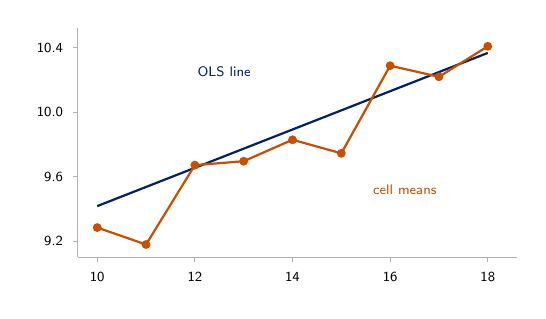
\begin{tikzpicture}[x=0.62cm, y=2.05cm]
  %% axes
  \draw[gray!60] (-0.4,0) -- (8.6,0);
  \draw[gray!60] (-0.4,0) -- (-0.4,1.42);
  \foreach \x/\l in {0/10, 2/12, 4/14, 6/16, 8/18}
    \draw[gray!60] (\x,0) -- (\x,-0.03) node[below,font=\tiny,text=black] {\l};
  \foreach \y/\l in {0.1/9.2, 0.5/9.6, 0.9/10.0, 1.3/10.4}
    \draw[gray!60] (-0.4,\y) -- (-0.5,\y) node[left,font=\tiny,text=black] {\l};
  %% OLS line
  \draw[dukeblue,thick] (0,0.318) -- (8,1.267);
  %% cell means
  \draw[accent,thick] (0,0.185) -- (1,0.080) -- (2,0.572) -- (3,0.596)
      -- (4,0.729) -- (5,0.645) -- (6,1.188) -- (7,1.119) -- (8,1.308);
  \foreach \p in {(0,0.185),(1,0.080),(2,0.572),(3,0.596),(4,0.729),
                  (5,0.645),(6,1.188),(7,1.119),(8,1.308)}
    \fill[accent] \p circle (1.6pt);
  \node[font=\tiny,accent] at (6.3,0.42) {cell means};
  \node[font=\tiny,dukeblue] at (2.6,1.15) {OLS line};
\end{tikzpicture}
\end{column}
\begin{column}{0.45\textwidth}
{\footnotesize
\begin{tabular}{@{}lcc@{}}
\toprule
step & actual & the line says \\
\midrule
$11\to12$ & \alert{$+0.49$} & $+0.12$ \\
$12\to13$ & $+0.02$ & $+0.12$ \\
$15\to16$ & \alert{$+0.54$} & $+0.12$ \\
$16\to17$ & \alert{$-0.07$} & $+0.12$ \\
\bottomrule
\end{tabular}}
\vskip6pt
{\footnotesize The returns are concentrated at the diploma years, 12 and 16.
The line spreads them evenly across all years. It misses the shape entirely:
it has no idea that 12 and 16 are special.}
\end{column}
\end{columns}
\vskip4pt
\alert{And yet we reported $0.119$ anyway.} What is that number?
\end{frame}

\begin{frame}{Estimating \emph{What}, Exactly?}
Look carefully at how we defined this estimator's target.
\vskip3pt
\begin{block}{The circularity}
We \emph{wrote down} $Y_i = \beta_0 + \beta_1 X_i + \epsilon_i$ and then showed
$\E[\hat\beta_1] = \beta_1$. But $\beta_1$ exists only because we assumed that
equation. If the CEF is not a line, and it is not, there is no true
$\beta_1$ for $\hat\beta_1$ to be unbiased \emph{for}.
\end{block}
\vskip3pt
\begin{itemize}\itemsep3pt
  \item \textbf{Estimand}: the population quantity you want. \quad
        \textbf{Estimator}: the recipe. \quad
        \textbf{Estimate}: the number.
  \item We have the last two. We have never named the first without assuming it
        into existence.
  \item Unbiasedness, consistency, standard errors are \alert{all statements
        about distance from a target.} No target, no statements.
\end{itemize}
\end{frame}

\begin{frame}{The Plan}
Define $\bm\beta$ as a feature of the \alert{joint distribution of $(Y_i, X_i)$}
, something that exists in every population, whether or not any line is true.
\vskip6pt
\begin{enumerate}\itemsep5pt
  \item The \textbf{CEF} $\E[Y_i\mid X_i]$: what we would most like to know.
        Assumption-free, and the answer to most sociological questions as
        actually posed.
  \item The \textbf{best linear predictor}: the line closest to the CEF. Defined
        for any joint distribution, no linearity assumed, none needed.
  \item A theorem connecting them, which tells us exactly what $0.119$ is a
        summary \emph{of}.
\end{enumerate}
\vskip6pt
\begin{alertblock}{Why this is worth an hour}
It converts ``your model is misspecified'' from a fatal objection into a
statement about \emph{approximation error}, which you can then evaluate,
bound, or fix by saturating. You cannot defend a regression you cannot say the
target of.
\end{alertblock}
\end{frame}

\begin{frame}{The Conditional Expectation Function (CEF)}
Everything so far was about a \emph{sample}. Step back to the population.
\vskip4pt
For an outcome $Y_i$ and covariates $X_i$, the \alert{conditional expectation
function} is
\begin{align*}
  g(x) \;=\; \E[Y_i \mid X_i = x] .
\end{align*}
\begin{itemize}\itemsep4pt
  \item In words: the average outcome among all units in the population with
        $X_i = x$, average earnings among people with exactly 16 years of
        schooling.
  \item This is what most sociological questions are really about: \emph{how does
        the average of $Y$ move as we move through the population along $X$?}
  \item Because $X_i$ is random, $\E[Y_i\mid X_i]$ is itself a random variable.
\end{itemize}
\end{frame}

\begin{frame}{Three Facts About the CEF}
\begin{block}{1. Law of iterated expectations}
$\E[Y_i] = \E\big[\E[Y_i\mid X_i]\big]$, the overall mean is the average of
the group means.
\end{block}
\pause
\begin{block}{2. CEF decomposition}
Define $\epsilon_i \equiv Y_i - \E[Y_i\mid X_i]$. Then $Y_i = \E[Y_i\mid X_i] + \epsilon_i$
with $\E[\epsilon_i\mid X_i] = 0$, and hence $\E[\epsilon_i m(X_i)] = 0$ for
\emph{any} function $m(\cdot)$.
\end{block}
\pause
\begin{block}{3. CEF prediction property}
$\E[Y_i\mid X_i] = \argmin_{m(\cdot)} \E\big[(Y_i - m(X_i))^2\big]$: among
\emph{all} functions of $X_i$, the CEF is the best mean-squared-error predictor.
\end{block}
\vskip2pt
\alert{These are identities, not assumptions.} They carry no causal content
whatever.
\end{frame}

\begin{frame}{Proof of the Decomposition Property\adv}
By definition $\epsilon_i = Y_i - \E[Y_i\mid X_i]$, so
\begin{align*}
  \E[\epsilon_i \mid X_i]
  = \E\big[Y_i \mid X_i\big] - \E[Y_i\mid X_i] = 0 .
\end{align*}
For any function $m(\cdot)$, apply the law of iterated expectations:
\begin{align*}
  \E\big[\epsilon_i\, m(X_i)\big]
  = \E\Big[\, \E\big[\epsilon_i\, m(X_i) \mid X_i \big] \Big]
  = \E\Big[ m(X_i)\, \underbrace{\E[\epsilon_i \mid X_i]}_{=\,0} \Big]
  = 0 . \quad\blacksquare
\end{align*}
\vskip4pt
Any random variable splits into a part \emph{explained} by $X_i$ and a part
orthogonal to \emph{every} function of $X_i$.
\end{frame}

\begin{frame}{Proof of the Prediction Property\adv}
For any candidate predictor $m(X_i)$, add and subtract the CEF:
\begin{align*}
  \E\big[(Y_i - m(X_i))^2\big]
  &= \E\Big[\big\{ (Y_i - \E[Y_i\mid X_i]) + (\E[Y_i\mid X_i] - m(X_i)) \big\}^2\Big]\\[2pt]
  &= \underbrace{\E\big[(Y_i-\E[Y_i\mid X_i])^2\big]}_{\text{does not involve } m}
   + \underbrace{\E\big[(\E[Y_i\mid X_i] - m(X_i))^2\big]}_{\geq\, 0}\\
  &\quad + 2\,\underbrace{\E\big[\epsilon_i\,(\E[Y_i\mid X_i]-m(X_i))\big]}_{=\,0
    \text{ by decomposition}} .
\end{align*}
The middle term is minimized at zero by setting $m(X_i)=\E[Y_i\mid X_i]$.
$\blacksquare$
\end{frame}

\begin{frame}{The Population Regression, or Best Linear Predictor}
The CEF is a general function and typically unknown. Restrict attention to
\emph{linear} predictors and define
\begin{align*}
  \bm\beta = \argmin_{b} \E\big[(Y_i - X_i'b)^2\big]
  \quad\Longrightarrow\quad
  \E\big[X_i(Y_i - X_i'\bm\beta)\big] = 0 .
\end{align*}
This is the population counterpart of the normal equations. In the bivariate case
it is exactly what you expect:
\begin{align*}
  \beta_1 = \frac{\Cov(X_i, Y_i)}{\Var(X_i)},
  \qquad
  \beta_0 = \E[Y_i] - \beta_1 \E[X_i] .
\end{align*}
\vskip4pt
Defining $e_i \equiv Y_i - X_i'\bm\beta$, we get $\E[X_ie_i]=0$
\alert{by construction}, in every population. Again: algebra, not causality.
\end{frame}

\begin{frame}{Why Should We Care About the Best \emph{Linear} Predictor?}
Three standard justifications \srcp{Angrist and Pischke 2009}:
\begin{enumerate}\itemsep6pt
  \item \textbf{If the CEF is linear}, the population regression \emph{is} the CEF.
  \item \textbf{If the CEF is nonlinear}, $X_i'\bm\beta$ is the minimum-MSE linear
        approximation to it:
        $\bm\beta = \argmin_b \E\big[(\E[Y_i\mid X_i] - X_i'b)^2\big]$.
  \item \textbf{Regardless}, $X_i'\bm\beta$ is the minimum-MSE linear predictor
        of $Y_i$.
\end{enumerate}
\vskip6pt
\pause
Justification 2 is the useful one in practice. OLS is a \emph{well-defined
summary of the CEF} even when you do not believe the CEF is a line, so
``the model is wrong'' is not, by itself, a fatal objection.
\end{frame}

\begin{frame}{Proof of the Regression-CEF Theorem\adv}
Claim: $\bm\beta = \argmin_b \E[(Y_i - X_i'b)^2]$ also solves
$\argmin_b \E\big[(\E[Y_i\mid X_i] - X_i'b)^2\big]$.
\begin{align*}
  \E[(Y_i - X_i'b)^2]
  &= \E\Big[\big\{ (Y_i - \E[Y_i\mid X_i]) + (\E[Y_i\mid X_i] - X_i'b)\big\}^2 \Big] \\
  &= \underbrace{\E\big[(Y_i - \E[Y_i\mid X_i])^2\big]}_{\text{free of } b}
  \;+\; \E\big[(\E[Y_i\mid X_i] - X_i'b)^2\big] \\
  &\quad + 2\,\underbrace{\E\big[\epsilon_i\,(\E[Y_i\mid X_i] - X_i'b)\big]}_{=\,0}
\end{align*}
The two objectives differ by a constant, so they share a minimizer.
$\blacksquare$
\end{frame}

\begin{frame}{Saturated Models: When Regression Is the CEF}
Suppose $X_i$ is \emph{discrete} with $J$ cells. Include a full set of $J-1$
dummies plus a constant. The regression is then \alert{saturated}: one free
parameter per cell.
\vskip6pt
\begin{itemize}\itemsep4pt
  \item A saturated regression reproduces the CEF \emph{exactly}, cell by cell.
        No functional-form assumption is being made at all.
  \item Example: regress log earnings on a dummy for each value of \texttt{educ}.
        The fitted values \emph{are} the cell means.
  \item Contrast: entering \texttt{educ} linearly imposes a constant increment,
        and is therefore an approximation.
\end{itemize}
\vskip4pt
\begin{block}{Practical upshot}
Whenever you can afford the degrees of freedom, saturating in the key covariate
is a free robustness check on functional form. We do this in lab.
\end{block}
\end{frame}

\begin{frame}{What That Detour Bought Us: Two Questions, Kept Apart}
Every argument about a regression coefficient is one of two questions. Keep them
apart and most confusion dissolves.
\vskip2pt
\begin{columns}[T]
\begin{column}{0.48\textwidth}
\begin{block}{Q1. What does $\hat\beta_1$ estimate?}
{\footnotesize
The minimum-MSE linear approximation to the CEF.
\vskip3pt
\alert{Always answerable}, algebra, true in every population.
\vskip3pt
``Your model is misspecified'' attacks this, and usually \emph{fails}: OLS has an
honest answer.}
\end{block}
\end{column}
\begin{column}{0.48\textwidth}
\begin{block}{Q2. Is \emph{that} the causal effect?}
{\footnotesize
Only if the units being compared are comparable.
\vskip3pt
\alert{Never answerable by algebra}, a claim about how the data came to be.
\vskip3pt
``Your treated and controls differ'' attacks this, and usually \emph{lands}:
nothing can repair it.}
\end{block}
\end{column}
\end{columns}
\vskip6pt
\pause
\alert{Weeks 1--4 are Q1. Weeks 5--13 are Q2.} That is the whole course.
\end{frame}

%%%%%%%%%%%%%%%%%%%%%%%%%%%%%%%%%%%%%%%%%%%%%%%%%%%%%%%%%%%%%%%%%%%%%%%%%%%%%%%
\section[Matrix Form]{The Matrix Form and Its Geometry}
%%%%%%%%%%%%%%%%%%%%%%%%%%%%%%%%%%%%%%%%%%%%%%%%%%%%%%%%%%%%%%%%%%%%%%%%%%%%%%%
\begin{frame}\sectionpage\end{frame}

\begin{frame}{Why Bother}
\begin{itemize}\itemsep5pt
  \item With $k$ regressors, scalar algebra needs $k$ normal equations and becomes
        unreadable. Matrix algebra stays two lines long for any $k$.
  \item The \alert{geometry}, projection onto a subspace, is invisible in
        scalar form and obvious in matrix form.
  \item Every estimator later in the course (fixed effects, IV, 2SLS, ridge,
        weighting, double ML) is a small variation on
        $\bhat = (\X'\X)^{-1}\X'\Y$. You will not be able to read the literature
        without it.
\end{itemize}
\vskip6pt
\begin{alertblock}{But}
Nothing in this section is new content. It is the \emph{same} normal equations
you already derived, written more compactly. Thursday's lab reviews every piece
of linear algebra we use.
\end{alertblock}
\end{frame}

\begin{frame}{Stacking the Data}
For $n$ units and $k$ regressors (including the constant):
\begin{align*}
  \Y = \begin{bmatrix} Y_1 \\ \vdots \\ Y_n \end{bmatrix}_{n\times 1},
  \quad
  \X = \begin{bmatrix} X_1' \\ \vdots \\ X_n' \end{bmatrix}
     = \begin{bmatrix}
        1 & X_{11} & \cdots & X_{1,k-1}\\
        \vdots & \vdots & & \vdots \\
        1 & X_{n1} & \cdots & X_{n,k-1}
       \end{bmatrix}_{n\times k},
  \quad
  \bm\epsilon = \begin{bmatrix} \epsilon_1 \\ \vdots \\ \epsilon_n\end{bmatrix}.
\end{align*}
The model, stacked over units:
\begin{align*}
  \Y = \X\bm\beta + \bm\epsilon
  \qquad\Longleftrightarrow\qquad
  Y_i = X_i'\bm\beta + \epsilon_i,\quad i=1,\dots,n .
\end{align*}
Two objects do all the work:
$\ \X'\X = \sum_i X_iX_i'$ (a $k\times k$ matrix) and
$\ \X'\Y = \sum_i X_i Y_i$ (a $k\times 1$ vector).
\end{frame}

\begin{frame}{Least Squares in Matrix Form}
\begin{align*}
  S(b) = \sum_{i} (Y_i - X_i'b)^2 = (\Y-\X b)'(\Y-\X b)
       = \Y'\Y - 2\,b'\X'\Y + b'\X'\X b .
\end{align*}
\pause
Differentiate, using $\partial (a'b)/\partial b = a$ and
$\partial (b'Ab)/\partial b = 2Ab$ for symmetric $A$:
\begin{align*}
  \frac{\partial S(b)}{\partial b} = -2\X'\Y + 2\X'\X b \overset{!}{=} 0
  \quad\Longrightarrow\quad
  \underbrace{\X'\X\,\bhat = \X'\Y}_{\text{\alert{normal equations}}} .
\end{align*}
\pause
These are the \emph{same} $k$ equations you wrote out one at a time. The
second-order condition holds because $\X'\X \succeq 0$, so $S$ is convex and any
stationary point is a global minimum.
\end{frame}

\begin{frame}{The Estimator, Existence, and Rank}
\begin{block}{The OLS estimator}
If $\rank(\X)=k$ (\emph{full column rank}), $\X'\X$ is invertible and
\begin{align*}
  \bhat = (\X'\X)^{-1}\X'\Y = \big(\En[X_iX_i']\big)^{-1}\En[X_iY_i] .
\end{align*}
\end{block}
\begin{itemize}\itemsep3pt
  \item Full column rank requires $n \geq k$ and no exact linear dependence among
        columns. It is the matrix version of ``$X$ must vary.''
  \item Failures you will actually meet: the \emph{dummy variable trap}; including
        a variable and a rescaling of it; a group indicator constant within a
        fixed effect.
  \item If rank fails, \texttt{R} silently drops a column and reports \texttt{NA}.
        That \texttt{NA} is never a mystery.
\end{itemize}
\end{frame}

\begin{frame}{Sanity Check: Recovering the Scalar Formula\adv}
Let $k=2$ with $X_i = (1, X_i)'$. Then
\begin{align*}
  \X'\X = \begin{bmatrix} n & \sum_i X_i \\ \sum_i X_i & \sum_i X_i^2\end{bmatrix},
  \qquad
  \X'\Y = \begin{bmatrix} \sum_i Y_i \\ \sum_i X_i Y_i \end{bmatrix} .
\end{align*}
Using $\begin{bmatrix} a & b\\ c& d\end{bmatrix}^{-1}
= \frac{1}{ad-bc}\begin{bmatrix} d & -b\\ -c & a\end{bmatrix}$,
\begin{align*}
  \hat\beta_1 = \frac{n\sum_i X_iY_i - \sum_i X_i \sum_i Y_i}
                     {n\sum_i X_i^2 - (\sum_i X_i)^2}
  = \frac{\Cov_n(X,Y)}{\Var_n(X)},
  \qquad
  \hat\beta_0 = \bar Y - \hat\beta_1 \bar X .
\end{align*}
\vskip4pt
Exactly what we derived by hand. The matrix form is a change of language, not of
substance.
\end{frame}

\begin{frame}{OLS Is a Projection\adv}
Think of $\Y$ as a single point in $\R^n$, one dimension per
\emph{observation}. The $k$ columns of $\X$ span a $k$-dimensional subspace
\begin{align*}
  \pcol(\X) = \{\X b : b \in \R^k\} \subset \R^n .
\end{align*}
OLS finds the point in $\pcol(\X)$ closest to $\Y$:
$\ \hat\Y = \argmin_{v \in \pcol(\X)} \|\Y - v\|^2$.
\vskip4pt
\begin{block}{Projection and annihilator matrices}
\begin{align*}
  \Pm = \X(\X'\X)^{-1}\X' \ (\text{``hat matrix''}),
  \qquad
  \Mm = \Ix_n - \Pm \ (\text{``residual maker''})
\end{align*}
so that $\hat\Y = \Pm\Y$ and $\ehat = \Mm\Y$.
\end{block}
\end{frame}

\begin{frame}{The Picture\adv}
\begin{center}
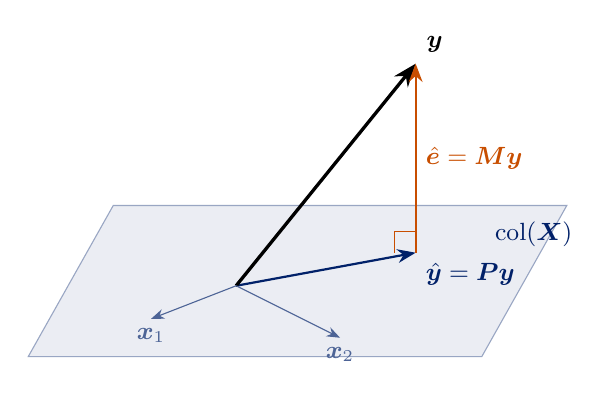
\begin{tikzpicture}[scale=1.2,>=Stealth]
  \fill[dukeblue!8] (-2.2,-0.75) -- (2.6,-0.75) -- (3.5,0.85) -- (-1.3,0.85) -- cycle;
  \draw[dukeblue!40] (-2.2,-0.75) -- (2.6,-0.75) -- (3.5,0.85) -- (-1.3,0.85) -- cycle;
  \node[dukeblue] at (3.15,0.55) {\small $\pcol(\X)$};
  \coordinate (O) at (0,0);
  \coordinate (Yhat) at (1.9,0.35);
  \coordinate (Y) at (1.9,2.35);
  \draw[->,thick,dukeblue] (O) -- (Yhat) node[below right] {\small $\hat{\bm{y}} = \bm{P}\bm{y}$};
  \draw[->,very thick] (O) -- (Y) node[above right] {\small $\bm{y}$};
  \draw[->,thick,accent] (Yhat) -- (Y) node[midway,right] {\small $\hat{\bm{e}} = \bm{M}\bm{y}$};
  \draw[accent] ($(Yhat)+(0,0.22)$) -- ($(Yhat)+(-0.22,0.22)$) -- ($(Yhat)+(-0.22,0)$);
  \draw[->,dukeblue!70] (O) -- (-0.9,-0.35) node[below] {\small $\bm{x}_1$};
  \draw[->,dukeblue!70] (O) -- (1.1,-0.55) node[below] {\small $\bm{x}_2$};
\end{tikzpicture}
\end{center}
\vskip-8pt
\begin{itemize}
  \item $\ehat \perp \pcol(\X)$, the geometric content of $\X'\ehat=\zero$, which
        is the geometric content of ``residuals are uncorrelated with the
        regressors.''
  \item Fitting is dropping a perpendicular. Everything else is bookkeeping.
\end{itemize}
\end{frame}

\begin{frame}{Properties of $\Pm$ and $\Mm$\adv}
\begin{columns}[T]
\begin{column}{0.48\textwidth}
\textbf{Symmetric}
\begin{align*}
  \Pm' = \Pm, \qquad \Mm' = \Mm
\end{align*}
\textbf{Idempotent}
\begin{align*}
  \Pm\Pm &= \X(\X'\X)^{-1}\underbrace{\X'\X(\X'\X)^{-1}}_{\Ix}\X' = \Pm\\
  \Mm\Mm &= (\Ix-\Pm)(\Ix-\Pm) = \Mm
\end{align*}
\textbf{Mutually orthogonal}
\begin{align*}
  \Pm\Mm = \Pm - \Pm\Pm = \zero
\end{align*}
\end{column}
\begin{column}{0.48\textwidth}
\textbf{Act correctly on $\X$}
\begin{align*}
  \Pm\X = \X, \qquad \Mm\X = \zero
\end{align*}
\textbf{Traces $=$ dimensions}
\begin{align*}
  \trace(\Pm) &= \trace\big((\X'\X)^{-1}\X'\X\big) = k\\
  \trace(\Mm) &= n - k
\end{align*}
\textbf{Eigenvalues} are all $0$ or $1$; $\Pm$ has $k$ ones, $\Mm$ has $n-k$.
\end{column}
\end{columns}
\vskip2pt
{\footnotesize Used repeatedly: $\trace(ABC)=\trace(BCA)$ (cyclic property).}
\end{frame}

\begin{frame}{Leverage\adv}
The $i$th diagonal element of $\Pm$,
\begin{align*}
  h_{ii} = X_i'(\X'\X)^{-1}X_i = \frac{\partial \hat Y_i}{\partial Y_i},
\end{align*}
is the \alert{leverage} of observation $i$: how much unit $i$'s own outcome pulls
its own fitted value.
\begin{itemize}\itemsep3pt
  \item $0 \leq h_{ii} \leq 1$ and $\sum_i h_{ii} = k$, so average leverage is
        $k/n$.
  \item High leverage means unusual \emph{covariate} values, not an unusual
        outcome.
  \item $\Var(\hat e_i) = \sigma^2(1-h_{ii})$: high-leverage points have
        artificially small residuals, they drag the line toward themselves.
  \item Leverage returns next week in the finite-sample corrections HC2 and HC3.
\end{itemize}
\end{frame}

\begin{frame}{Sums of Squares, Again\adv}
Because $\Y = \Pm\Y + \Mm\Y$ and $\Pm\Mm=\zero$, Pythagoras gives
\begin{align*}
  \Y'\Y = \Y'\Pm\Y + \Y'\Mm\Y = \hat\Y'\hat\Y + \ehat'\ehat .
\end{align*}
Subtracting $n\bar Y^2$ (valid when a constant is included) returns the scalar
decomposition $TSS = ESS + RSS$.
\vskip6pt
\begin{itemize}
  \item $R^2$ is also $\cos^2$ of the angle between $\Y - \bar Y\one$ and
        $\hat\Y - \bar Y\one$: fit is literally about angles.
  \item Adding a regressor enlarges $\pcol(\X)$, which can only move $\hat\Y$
        closer to $\Y$, the geometric reason $R^2$ never falls.
\end{itemize}
\end{frame}

%%%%%%%%%%%%%%%%%%%%%%%%%%%%%%%%%%%%%%%%%%%%%%%%%%%%%%%%%%%%%%%%%%%%%%%%%%%%%%%
\section[Properties]{Statistical Properties of OLS}
%%%%%%%%%%%%%%%%%%%%%%%%%%%%%%%%%%%%%%%%%%%%%%%%%%%%%%%%%%%%%%%%%%%%%%%%%%%%%%%
\begin{frame}\sectionpage\end{frame}

\begin{frame}{The Classical Assumptions}
\begin{enumerate}\itemsep3pt
  \item[\textbf{A1}] \textbf{Linearity in parameters}: $Y_i = X_i'\bm\beta + \epsilon_i$.
        (Not restrictive: $X$ may contain logs, powers, splines, interactions.)
  \item[\textbf{A2}] \textbf{Random sampling}: $(Y_i,X_i)$ i.i.d.\ from the population.
  \item[\textbf{A3}] \textbf{No perfect collinearity}: $X$ genuinely varies;
        $\rank(\X)=k$.
  \item[\textbf{A4}] \textbf{Strict exogeneity}: $\E[\epsilon_i \mid X_i] = 0$.
  \item[\textbf{A5}] \textbf{Spherical errors}: $\Var(\epsilon_i\mid \X)=\sigma^2$
        for all $i$ (homoskedasticity), and $\Cov(\epsilon_i,\epsilon_j\mid\X)=0$
        for $i\neq j$ (no correlation across units).
  \item[\textbf{A6}] \textbf{Normality} (optional):
        $\epsilon_i\mid X_i \sim \mathcal{N}(0,\sigma^2)$.
\end{enumerate}
\vskip2pt
\begin{block}{What each buys you}
A1--A4 $\Rightarrow$ unbiasedness. $+$A5 $\Rightarrow$ the simple variance formula
and Gauss--Markov efficiency. $+$A6 $\Rightarrow$ exact $t$ and $F$ in finite
samples. \\
\alert{Week 2 drops A5. Weeks 5+ interrogate A4, the only one that matters for
causality.}
\end{block}
\end{frame}

\begin{frame}{Unbiasedness, in Scalar Form}
Take the bivariate case. Start from the slope formula and substitute
$Y_i = \beta_0+\beta_1X_i+\epsilon_i$:
\begin{align*}
  \hat\beta_1
  &= \frac{\sum_i (X_i-\bar X)(Y_i - \bar Y)}{\sum_i (X_i - \bar X)^2}
   = \frac{\sum_i (X_i-\bar X)\big(\beta_1(X_i - \bar X) + (\epsilon_i - \bar\epsilon)\big)}
          {\sum_i (X_i - \bar X)^2} \\[4pt]
  &= \beta_1 + \frac{\sum_i (X_i - \bar X)\epsilon_i}{\sum_i (X_i-\bar X)^2} .
\end{align*}
\pause
\begin{alertblock}{Remember this line}
$\hat\beta_1 = \beta_1 + (\text{a weighted average of the errors})$. Every result
about bias and variance in this course comes from staring at it.
\end{alertblock}
Taking expectations conditional on $X$ and using A4 ($\E[\epsilon_i\mid X]=0$)
gives $\E[\hat\beta_1\mid X]=\beta_1$, and hence $\E[\hat\beta_1]=\beta_1$.
\end{frame}

\begin{frame}{Unbiasedness, in Matrix Form\adv}
The same two lines, for any $k$:
\begin{align*}
  \bhat &= (\X'\X)^{-1}\X'(\X\bm\beta + \bm\epsilon)
         = \bm\beta + (\X'\X)^{-1}\X'\bm\epsilon , \\[4pt]
  \E[\bhat\mid\X] &= \bm\beta + (\X'\X)^{-1}\X'\underbrace{\E[\bm\epsilon\mid\X]}_{=\,\zero}
  = \bm\beta . \qquad\blacksquare
\end{align*}
\vskip6pt
\begin{itemize}
  \item Note where the work is done: \emph{only} by A4.
  \item Heteroskedasticity, clustering, and non-normality do \alert{not} bias
        $\bhat$. They affect its \emph{variance}, next week.
  \item A4 fails whenever an omitted variable, reverse causation, measurement
        error in $X$, or selection puts something correlated with $X$ into
        $\epsilon$. That is the entire causal-inference problem in one sentence.
\end{itemize}
\end{frame}

\begin{frame}{The Variance of $\hat\beta_1$, in Scalar Form}
From $\hat\beta_1 - \beta_1 = \dfrac{\sum_i (X_i - \bar X)\epsilon_i}{\sum_i (X_i-\bar X)^2}$,
and treating $X$ as fixed:
\begin{align*}
  \Var(\hat\beta_1\mid X)
  = \frac{\sum_i (X_i-\bar X)^2\,\Var(\epsilon_i\mid X)}
         {\big[\sum_i (X_i - \bar X)^2\big]^2}
\end{align*}
using only that the $\epsilon_i$ are uncorrelated across units.
\pause
\vskip4pt
Under homoskedasticity (A5), $\Var(\epsilon_i\mid X)=\sigma^2$ factors out:
\begin{align*}
  \boxed{\;\Var(\hat\beta_1\mid X) = \frac{\sigma^2}{\sum_i (X_i - \bar X)^2}\;}
\end{align*}
\alert{Keep the first expression in view.} Next week we simply refuse to assume
$\Var(\epsilon_i\mid X)$ is constant, and that is all a ``robust standard
error'' is.
\end{frame}

\begin{frame}{What Drives Precision}
\begin{align*}
  \Var(\hat\beta_1\mid X) = \frac{\sigma^2}{\sum_i (X_i - \bar X)^2}
  = \frac{\sigma^2}{n\,\Var_n(X)} ,
\end{align*}
and with more regressors,
$\Var(\hat\beta_j) = \dfrac{\sigma^2}{n\,\Var_n(X_j)\,(1-R_j^2)}$
where $R_j^2$ is from regressing $X_j$ on the other regressors.
\vskip2pt
\begin{itemize}\itemsep2pt
  \item \textbf{Noise} $\sigma^2$ up $\Rightarrow$ variance up.
  \item \textbf{Sample size} $n$ up $\Rightarrow$ variance down like $1/n$;
        standard error down like $1/\sqrt n$.
  \item \textbf{Spread of $X$} up $\Rightarrow$ variance down.
  \item \textbf{Collinearity} $R_j^2 \to 1$ $\Rightarrow$ variance explodes; the
        \emph{variance inflation factor} is $1/(1-R_j^2)$.
\end{itemize}
\vskip3pt
Collinearity violates no assumption. It says the data contain little independent
information about $\beta_j$.
\end{frame}

\begin{frame}{Estimating $\sigma^2$}
$\sigma^2 = \E[\epsilon_i^2]$ is unknown; we have residuals, not errors. The
natural estimator is
\begin{align*}
  s^2 = \frac{1}{n-k}\sum_i \hat e_i^2 ,
  \qquad \E[s^2] = \sigma^2 .
\end{align*}
\begin{itemize}\itemsep3pt
  \item Why $n-k$ and not $n$? The residuals satisfy $k$ linear constraints
        (the normal equations), so they are systematically ``too short.''
  \item In matrix form\adv: $\ehat = \Mm\bm\epsilon$, so
        $\E[\ehat'\ehat] = \sigma^2\trace(\Mm) = \sigma^2(n-k)$.
  \item Then $\hat{V}(\hat\beta_1) = s^2/\sum_i (X_i-\bar X)^2$, whose
        square root is the standard error your software prints.
\end{itemize}
\end{frame}

\begin{frame}{The Gauss--Markov Theorem\adv}
\begin{block}{Theorem}
Under A1--A5, $\bhat$ is the \alert{Best Linear Unbiased Estimator}: among all
$\tilde{\bm\beta} = \bm{C}\Y$ with $\bm C$ a function of $\X$ and
$\E[\tilde{\bm\beta}\mid\X]=\bm\beta$,
$\Var(\tilde{\bm\beta}\mid\X) - \Var(\bhat\mid\X) \succeq 0$.
\end{block}
\pause
\textbf{Proof.} Write $\bm{C} = (\X'\X)^{-1}\X' + \bm{D}$. Unbiasedness for all
$\bm\beta$ forces $\bm{D}\X = \zero$. Then
\begin{align*}
  \Var(\bm C\Y\mid\X)
  &= \sigma^2\big[(\X'\X)^{-1}\X' + \bm D\big]\big[\X(\X'\X)^{-1} + \bm D'\big] \\
  &= \sigma^2(\X'\X)^{-1}
   + \sigma^2\underbrace{(\X'\X)^{-1}\X'\bm D'}_{=\,\zero}
   + \sigma^2\underbrace{\bm D\X(\X'\X)^{-1}}_{=\,\zero}
   + \sigma^2\bm{D}\bm{D}' \\
  &= \Var(\bhat\mid\X) + \sigma^2\bm{D}\bm{D}' \succeq \Var(\bhat\mid\X) .
  \qquad\blacksquare
\end{align*}
\end{frame}

\begin{frame}{Reading Gauss--Markov Correctly}
\begin{itemize}\itemsep5pt
  \item ``Best'' only \alert{within the class of linear unbiased} estimators.
        Biased estimators (ridge, lasso, shrinkage) can have far lower mean
        squared error, Week 12.
  \item Efficiency requires A5. Under heteroskedasticity OLS stays unbiased but is
        no longer BLUE; weighted least squares with the correct weights is.
  \item In practice we rarely know the weights, so we keep OLS and fix the
        \emph{standard errors} instead, the entire subject of next week.
  \item Gauss--Markov says nothing about causality. It is a statement about the
        variance of an estimator for the population regression coefficient,
        whatever that coefficient happens to mean.
\end{itemize}
\end{frame}

\begin{frame}{Finite-Sample Distribution Under Normality}
If A6 also holds, then conditional on $X$,
\begin{align*}
  \hat\beta_1 \sim \mathcal{N}\Big(\beta_1,\ \tfrac{\sigma^2}{\sum_i (X_i-\bar X)^2}\Big),
  \qquad
  \frac{(n-k)s^2}{\sigma^2} \sim \chi^2_{n-k},
  \qquad
  \hat\beta_1 \indep s^2 ,
\end{align*}
so that
$t = \dfrac{\hat\beta_1 - \beta_1}{\mathrm{se}(\hat\beta_1)} \sim t_{n-k}$.
\vskip6pt
\begin{itemize}
  \item $\hat\beta_1$ is a \emph{linear} function of the errors, hence normal when
        they are.
  \item Without A6, all of this holds only \emph{approximately}, and only for
        large $n$. That is next week.
\end{itemize}
\end{frame}

%%%%%%%%%%%%%%%%%%%%%%%%%%%%%%%%%%%%%%%%%%%%%%%%%%%%%%%%%%%%%%%%%%%%%%%%%%%%%%%
\section[Partialling Out]{Partialling Out in General}
%%%%%%%%%%%%%%%%%%%%%%%%%%%%%%%%%%%%%%%%%%%%%%%%%%%%%%%%%%%%%%%%%%%%%%%%%%%%%%%
\begin{frame}\sectionpage\end{frame}

\begin{frame}{The Frisch--Waugh--Lovell Theorem\adv}
Partition $\X = [\,\X_1\ \ \X_2\,]$: a treatment of interest and controls.
Let $\Mm_2 = \Ix - \X_2(\X_2'\X_2)^{-1}\X_2'$ and define
\begin{align*}
  \tilde{\X}_1 = \Mm_2\X_1 ,
  \qquad
  \tilde{\Y} = \Mm_2\Y .
\end{align*}
\begin{block}{Theorem}
The OLS estimate $\hat{\bm\beta}_1$ from the full regression equals
\begin{align*}
  \hat{\bm\beta}_1 = (\tilde\X_1'\tilde\X_1)^{-1}\tilde\X_1'\tilde\Y
                   = (\tilde\X_1'\tilde\X_1)^{-1}\tilde\X_1'\Y ,
\end{align*}
and the residuals from the short regression are numerically identical to $\ehat$
from the full one.
\end{block}
\vskip2pt
This is the three-step recipe from earlier, now for any number of controls.
\end{frame}

\begin{frame}{Proof of FWL\adv}
Premultiply the model by $\Mm_2$ and use $\Mm_2\X_2 = \zero$:
\begin{align*}
  \Mm_2\Y = \Mm_2\X_1\bm\beta_1 + \underbrace{\Mm_2\X_2}_{=\zero}\bm\beta_2
          + \Mm_2\bm\epsilon
  \quad\Longrightarrow\quad
  \tilde\Y = \tilde\X_1\bm\beta_1 + \Mm_2\bm\epsilon .
\end{align*}
\pause
For the estimator, decompose the fitted model
$\Y = \X_1\hat{\bm\beta}_1 + \X_2\hat{\bm\beta}_2 + \ehat$ and premultiply by
$\tilde\X_1' = \X_1'\Mm_2$:
\begin{align*}
  \tilde\X_1'\Y
  = \tilde\X_1'\tilde\X_1\hat{\bm\beta}_1
  + \X_1'\underbrace{\Mm_2\X_2}_{=\zero}\hat{\bm\beta}_2
  + \underbrace{\X_1'\Mm_2\ehat}_{=\,0} ,
\end{align*}
using $\Mm_2\ehat = \ehat$ (since $\X_2'\ehat = \zero$) and $\X_1'\ehat = \zero$.
Solving gives the result. Using $\tilde\Y$ instead of $\Y$ changes nothing
because $\tilde\X_1'\Mm_2 = \tilde\X_1'$. $\blacksquare$
\end{frame}

\begin{frame}{Why FWL Matters More Than It Looks}
\begin{enumerate}\itemsep6pt
  \item \textbf{Interpretation.} ``Controlling for $W$'' $=$ discarding all
        covariance between $X_1$ and $W$. Your estimate lives on what remains.
  \item \textbf{Computation.} Fixed-effects estimators \emph{are} FWL: regressing
        on unit dummies is the same as demeaning within unit (Week 10).
  \item \textbf{Diagnostics.} The added-variable plot is the only two-dimensional
        picture that faithfully represents a multivariate slope.
  \item \textbf{Generality.} Nothing in the argument requires $\X_2$ to enter
        linearly, it only requires that we can compute the part of $X_1$ that
        $\X_2$ predicts. That observation is the seed of a large literature, and
        we return to it briefly in Week 13.
\end{enumerate}
\end{frame}

\begin{frame}{Omitted Variables, in Matrix Form\adv}
With $\X_1$ included and $\X_2$ omitted,
\begin{align*}
  \E[\tilde{\bm\beta}_1 \mid \X]
  = \bm\beta_1 + \underbrace{(\X_1'\X_1)^{-1}\X_1'\X_2}_{\hat{\bm\delta}}\,\bm\beta_2 .
\end{align*}
\begin{itemize}\itemsep4pt
  \item Each column of $\hat{\bm\delta}$ is the coefficient vector from regressing
        one omitted variable on all the included ones, exactly $\delta_1$ from
        the scalar case, stacked.
  \item With several omitted variables the bias is a \emph{sum} of terms which may
        offset, so ``the bias must be positive'' arguments require care.
  \item Sensitivity analysis (Week 6) formalizes the question: how strong would an
        omitted confounder have to be to overturn the result?
\end{itemize}
\end{frame}

%%%%%%%%%%%%%%%%%%%%%%%%%%%%%%%%%%%%%%%%%%%%%%%%%%%%%%%%%%%%%%%%%%%%%%%%%%%%%%%
\section[Adjustment]{Regression as Adjustment}
%%%%%%%%%%%%%%%%%%%%%%%%%%%%%%%%%%%%%%%%%%%%%%%%%%%%%%%%%%%%%%%%%%%%%%%%%%%%%%%
\begin{frame}\sectionpage\end{frame}

\begin{frame}{Regression With a Binary Treatment}
Let $D_i\in\{0,1\}$ be a treatment and $W_i$ controls:
\begin{align*}
  Y_i = \alpha + \rho D_i + W_i'\gamma + e_i .
\end{align*}
Suppose that \emph{within cells of $W_i$} treatment is as good as randomly
assigned. Then the cell-specific difference in means
\begin{align*}
  \tau(w) = \E[Y_i \mid D_i=1, W_i=w] - \E[Y_i\mid D_i = 0, W_i = w]
\end{align*}
is the causal effect in that cell.
\vskip4pt
\alert{Question}: when $\tau(w)$ varies across cells, what single number does OLS
report?
\end{frame}

\begin{frame}{OLS Reports a Variance-Weighted Average\adv}
If the model is saturated in $W_i$ \srcp{Angrist and Pischke 2009}:
\begin{align*}
  \rho = \frac{\E\big[\sigma_D^2(W_i)\,\tau(W_i)\big]}{\E\big[\sigma_D^2(W_i)\big]},
  \qquad \sigma_D^2(w) = \Var(D_i \mid W_i = w) = p(w)\big(1-p(w)\big),
\end{align*}
where $p(w) = \Pr(D_i=1\mid W_i=w)$ is the \emph{propensity score}.
\vskip6pt
\begin{itemize}\itemsep3pt
  \item OLS averages cell-level effects with weights proportional to the
        \alert{conditional variance of treatment}.
  \item Cells with $p(w)\approx 0.5$ dominate; cells where nearly everyone is (or
        is not) treated get almost no weight.
  \item So OLS does not generally deliver the ATE or the ATT, it delivers its
        own weighted average. Matching and weighting (Week 6) let you choose the
        weights deliberately.
\end{itemize}
\end{frame}

\begin{frame}{Good Controls, Bad Controls}
Adding a control is not automatically an improvement.
\vskip2pt
\begin{columns}[T]
\begin{column}{0.47\textwidth}
\textbf{Good controls}
\begin{itemize}
  \item Confounders: common causes of $D$ and $Y$.
  \item Pre-treatment covariates that predict $Y$ (precision gains).
\end{itemize}
\end{column}
\begin{column}{0.49\textwidth}
\textbf{Bad controls}
\begin{itemize}
  \item \alert{Post-treatment} variables (mediators): conditioning removes part of
        the effect you want.
  \item \alert{Colliders}: common effects of $D$ and $Y$; conditioning
        \emph{creates} association where none existed.
  \item Proxies for the outcome.
\end{itemize}
\end{column}
\end{columns}
\vskip4pt
\begin{alertblock}{Preview}
No algebra distinguishes these cases: the distinction is \emph{causal}, not
statistical. We need a language for causal assumptions, which is Week 5.
\end{alertblock}
\end{frame}

\begin{frame}{Where This Leaves Us}
\begin{itemize}\itemsep5pt
  \item OLS minimizes squared errors. Everything else, the slope formula, the
        normal equations, FWL, OVB, follows from that one criterion by algebra.
  \item In the population, OLS estimates the best linear approximation to the CEF.
        Under A1--A4 the sample version is unbiased for it.
  \item Whether that coefficient is a \emph{causal effect} is a separate question
        that regression cannot answer.
  \item \textbf{Next week}: we have $\hat\beta$; now we need to know how uncertain
        it is, and the standard error your software prints is usually the wrong
        one.
\end{itemize}
\vskip6pt
\begin{block}{Before Thursday}
Install \texttt{R} and \texttt{RStudio}; skim MHE Chapter 3 and CCI Chapter 6.
Lab covers the matrix algebra used today and OLS by hand.
\end{block}
\end{frame}

\begin{frame}{References}
\footnotesize
\begin{itemize}\itemsep3pt
\item Angrist, Joshua D. and J\"orn-Steffen Pischke. 2009.
\textit{Mostly Harmless Econometrics}. Princeton University Press. [Ch.\ 3]
\item Morgan, Stephen L. and Christopher Winship. 2015.
\textit{Counterfactuals and Causal Inference}, 2nd ed. Cambridge University Press.
[Ch.\ 6]
\item James, Gareth, Daniela Witten, Trevor Hastie, and Robert Tibshirani. 2021.
\textit{An Introduction to Statistical Learning}, 2nd ed. Springer. [Ch.\ 2--3]
\item Correll, Josh, Abigail M. Folberg, Charles M. Judd, Gary H. McClelland, and
Carey S. Ryan. 2024. \textit{Data Analysis: A Model Comparison Approach to
Regression, ANOVA, and Beyond}, 4th ed. Routledge. [for review]
\end{itemize}
\end{frame}

\end{document}
